\documentclass{article}

\usepackage{graphicx}
\usepackage{tikz}
\usepackage{tikzsymbols}
\usetikzlibrary{calc,patterns,shapes.geometric}
\pagestyle{empty}
\usepackage[margin=0pt]{geometry}
\geometry{papersize={14in,12in}}

\def\centerarc[#1](#2)(#3:#4:#5){\draw[#1] ($(#2)+({#5*cos(#3)},{#5*sin(#3)})$) arc (#3:#4:#5);}

\begin{document}
	\begin{figure}
		\centering
		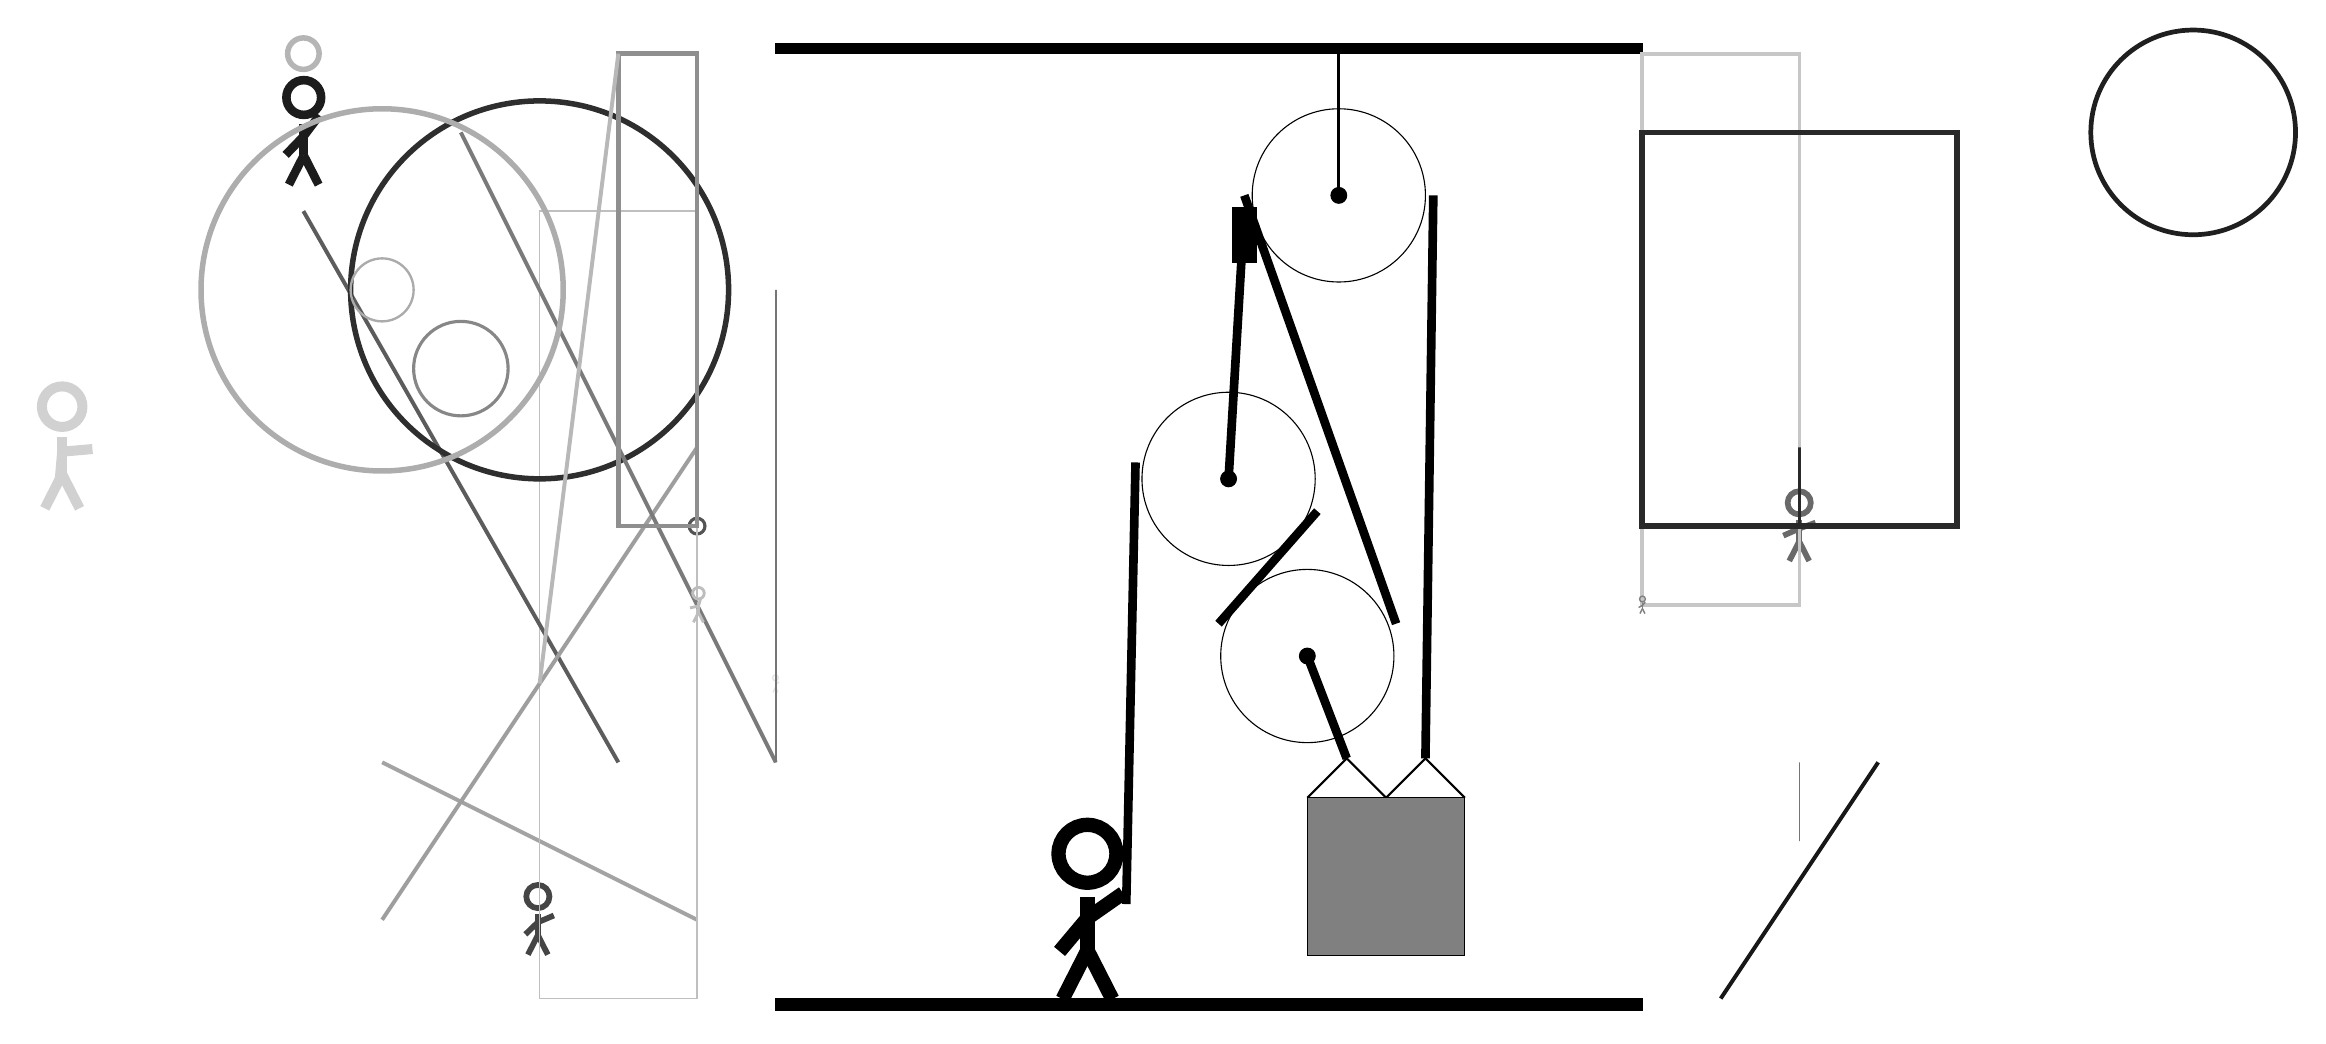
\begin{tikzpicture}
			%%%%% START %%%%%
			
			\draw[fill=black] (-6, 9) rectangle (5, 9.125);
			
			\draw (-0.25, 3.6) circle (1.1);
			\draw[fill=black] (-0.25, 3.6) circle (0.1);
			
			\draw (0.75, 1.35) circle (1.1);
			\draw[fill=black] (0.75, 1.35) circle (0.1);
			
			\draw (1.15, 7.2) circle (1.1);
			\draw[fill=black] (1.15, 7.2) circle (0.1);
			\draw[very thick] (1.15, 7.2) -- (1.15, 9);
			
			\draw[thick]  (0.75, -0.45) -- (1.25, 0.05) -- (1.75, -0.45) -- (2.25, 0.05) -- (2.75, -0.45);
			\draw[fill=black!50] (0.75, -0.45) rectangle (2.75, -2.45);
			
			\draw[line width=1.1mm] (-0.25, 3.6) -- (-0.05, 7.0);
			\draw[line width=1.1mm, fill=black](-0.15, 6.4) rectangle (0.05, 7.0);
			\draw[line width=1.1mm] (-1.55, -1.8) -- (-1.4318, 3.8083);
			\centerarc[line width=1.1mm](-0.25, 3.6)(-20:170:1.2000000000000002);
			\draw[line width=1.1mm] (0.8776, 3.1896) -- (-0.3776, 1.7604);
			\centerarc[line width=1.1mm](0.75, 1.35)(160:380:1.2000000000000002);
			\draw[line width=1.1mm] (1.8776, 1.7604) -- (-0.05, 7.2);
			\draw[line width=1.1mm](0.75, 1.35) -- (1.25, 0.05);
			\centerarc[line width=1.1mm](1.15, 7.2)(0:180:1.2000000000000002);
			\draw[line width=1.1mm] (2.35, 7.2) -- (2.25, 0.05);
			
			\node at (-2, -1.9) {\Strichmaxerl[10][50][35]};
			
			\node[line width=0.7mm, color=black!73] at (-9, -2) {\Strichmaxerl[4][44][23]};
			
			\draw [line width=0.7mm, color=black!29](-12, 9) circle (0.2);
			\draw[line width=0.5mm, color=black!91](6, -3) -- (8, 0);
			\node[line width=0.6mm, color=black!18] at (-15, 4) {\Strichmaxerl[7][85][5]};
			\draw[line width=0.5mm, color=black!36](-7, -2) -- (-11, 0);
			\draw[line width=0.2mm, color=black!54] (7, -1) rectangle (7, 0);
			\node[line width=0.2mm, color=black!59] at (7, 3) {\Strichmaxerl[4][24][20]};
			
			\draw [line width=0.6mm, color=black!88](12, 8) circle (1.3);
			\node[line width=0.6mm, color=black!10] at (-6, 1) {\Strichmaxerl[1][90][32]};
			\draw [line width=0.4mm, color=black!67](-7, 3) circle (0.1);
			
			\draw[line width=0.2mm, color=black!25] (-7, -3) rectangle (-9, 7);
			\draw[line width=0.5mm, color=black!64](-8, 0) -- (-12, 7);
			\node[line width=0.3mm, color=black!89] at (-12, 8) {\Strichmaxerl[6][46][53]};
			\draw[line width=0.5mm, color=black!22] (5, 9) rectangle (7, 2);
			\draw [line width=0.7mm, color=black!82](-9, 6) circle (2.4);
			\draw [line width=0.4mm, color=black!47](-10, 5) circle (0.6);
			\draw[line width=0.5mm, color=black!38](-11, -2) -- (-7, 4);
			
			\node[line width=0.2mm, color=black!50] at (5, 2) {\Strichmaxerl[1][28][50]};
			\draw[line width=0.5mm, color=black!52](-6, 0) -- (-10, 8);
			
			\draw[line width=0.2mm, color=black!54] (-6, 6) rectangle (-6, 0);
			\draw[line width=0.6mm, color=black!44] (-8, 9) rectangle (-7, 3);
			\draw[line width=0.7mm, color=black!84] (5, 3) rectangle (9, 8);
			\draw[line width=0.4mm, color=black!84] (7, 3) rectangle (7, 4);
			\draw[line width=0.5mm, color=black!28](-8, 9) -- (-9, 1);
			\draw [line width=0.7mm, color=black!32](-11, 6) circle (2.3);
			\draw [line width=0.3mm, color=black!33](-11, 6) circle (0.4);
			\node[line width=0.2mm, color=black!26] at (-7, 2) {\Strichmaxerl[2][12][74]};
			
			\draw[fill=black] (-6, -3) rectangle (5, -3.15);
			
			%%%%% END %%%%%
		\end{tikzpicture}
	\end{figure}	
\end{document}